%\documentclass[a4paper]{article}
%% Language and font encodings
\documentclass[twocolumn,aps,prl]{revtex4-1}
\usepackage[utf8]{inputenc}
\usepackage[spanish, es-tabla]{babel}
\usepackage[T1]{fontenc}
\usepackage{amsmath}
\usepackage{amssymb}
\usepackage{siunitx}
\usepackage{multirow}
\usepackage{float}
\usepackage{enumitem} % enumerar

\sisetup{math-micro=\text{µ},text-micro=µ}

\usepackage[toc,page]{appendix}

%% Sets page size and margins
\usepackage[a4paper,top=1.5cm,bottom=2cm,left=1.7cm,right=1.7cm,marginparwidth=1.75cm]{geometry}

%% Sets caption text size(its bigger than text)
\usepackage{caption}
\captionsetup[figure]{font=small}
\usepackage{subcaption}

%% Useful packages
\usepackage{svg}
\usepackage{epstopdf}
\usepackage{amsmath}
\usepackage{graphicx}
\usepackage[colorlinks=true, allcolors=blue]{hyperref}

\newcommand{\nstar}{n^*} 
\newcommand{\Nstar}{N^*} 

\newcommand*\sepline{%
  \begin{center}
    \rule[1ex]{.5\textwidth}{.5pt}
  \end{center}}

%%%%%%%%%%%%%%%%%%%%%%%%%%%%%%%%%%%%%%%%%%%%%%%%%%%%%%
%%%%%%%%%%%%%%%%%%%%%%%%%%%%%%%%%%%%%%%%%%%%%%%%%%%%%%
%%%%%%%%%%%%%%%%%%%%%%%%%%%%%%%%%%%%%%%%%%%%%%%%%%%%%%
%%%%%%%%%%%%%%%%%%%%%%%%%%%%%%%%%%%%%%%%%%%%%%%%%%%%%%
%%%%%%%%%%%%%%%%%%%%%%%%%%%%%%%%%%%%%%%%%%%%%%%%%%%%%%

\begin{document}

% ██   ██ ███████  █████  ██████
% ██   ██ ██      ██   ██ ██   ██
% ███████ █████   ███████ ██   ██
% ██   ██ ██      ██   ██ ██   ██
% ██   ██ ███████ ██   ██ ██████

\title{Práctico 2}
\author{M. G. Aramayo}
\affiliation{Matemática de sistemas biológicos, Instituto Balseiro}

% \begin{abstract}
% Mete acá las conclusiones.
% \end{abstract}

\maketitle


% ███████╗██╗  ██╗ ██╗
% ██╔════╝╚██╗██╔╝███║
% █████╗   ╚███╔╝ ╚██║
% ██╔══╝   ██╔██╗  ██║
% ███████╗██╔╝ ██╗ ██║
% ╚══════╝╚═╝  ╚═╝ ╚═╝

\section{Resolución Ej 1:}

% \begin{figure}
%     \centering
%     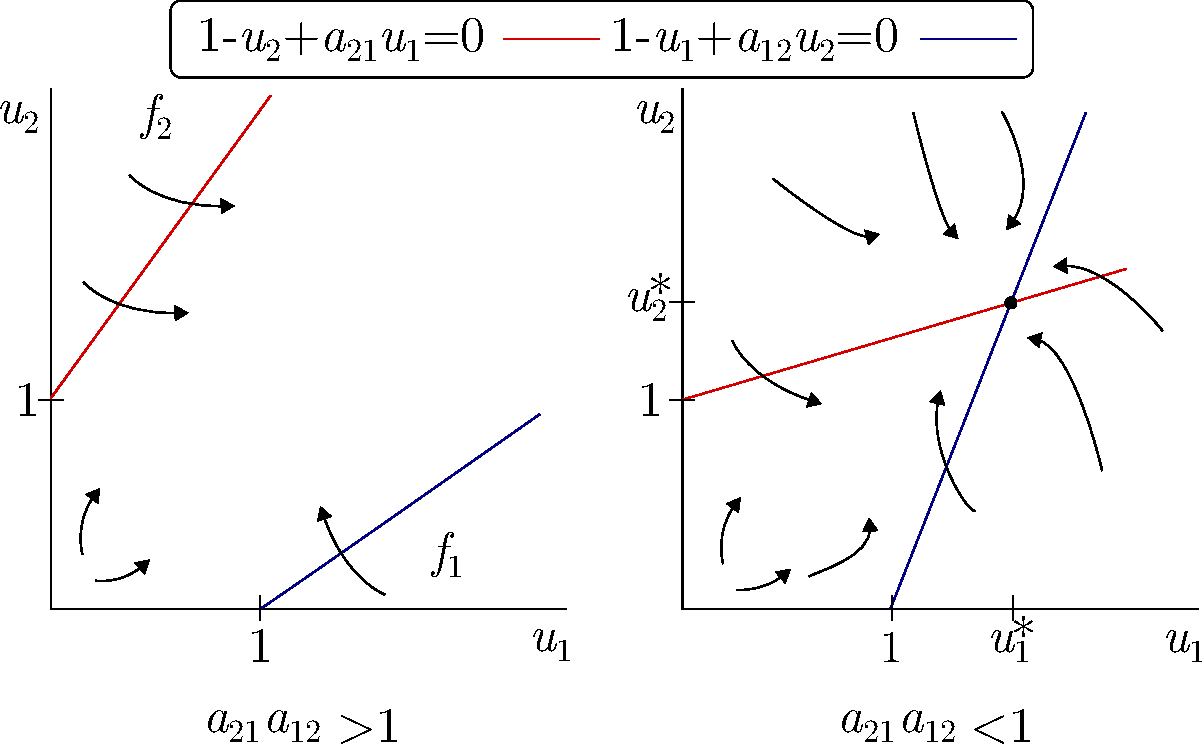
\includegraphics[width=0.5\textwidth]{figuras/equilibrio.pdf}
%     \caption{a.}
%     \label{fig:mosquitos}
% \end{figure}


% ███████╗██╗  ██╗    ██████╗  
% ██╔════╝╚██╗██╔╝    ╚════██╗
% █████╗   ╚███╔╝      █████╔╝
% ██╔══╝   ██╔██╗     ██╔═══╝ 
% ███████╗██╔╝ ██╗    ███████╗
% ╚══════╝╚═╝  ╚═╝    ╚══════╝

\section{Resolución Ej 2:}


%%%%%%%%%%%%%%%%%%%%%%%%%%%%%%%%%%%%%%%%%%%%%%%%%%%%%%%%%%%%%%%%%%%%%%
\sepline
%%%%%%%%%%%%%%%%%%%%%%%%%%%%%%%%%%%%%%%%%%%%%%%%%%%%%%%%%%%%%%%%%%%%%%


% ███████╗██╗  ██╗    ██████╗     
% ██╔════╝╚██╗██╔╝    ╚════██╗    
% █████╗   ╚███╔╝      █████╔╝    
% ██╔══╝   ██╔██╗      ╚═══██╗    
% ███████╗██╔╝ ██╗    ██████╔╝    
% ╚══════╝╚═╝  ╚═╝    ╚═════╝     

\section{Resolución Ej 3:}

% \bibliography{sample}

\end{document}

% ███    ██  ██████  ████████  █████  ███████
% ████   ██ ██    ██    ██    ██   ██ ██
% ██ ██  ██ ██    ██    ██    ███████ ███████
% ██  ██ ██ ██    ██    ██    ██   ██      ██
% ██   ████  ██████     ██    ██   ██ ███████


% ████████ ██    ██ ██████   ██████  ███████
%    ██     ██  ██  ██   ██ ██    ██ ██
%    ██      ████   ██████  ██    ██ ███████
%    ██       ██    ██      ██    ██      ██
%    ██       ██    ██       ██████  ███████

% atomico
% volumen
% parametro
% mantenia
% dielectrico
% perdida
% ferroelectrico
% difractograma
% difractometro
% minimo
% maximo
% tension
% conversion
% aislacion
% medicion
% resolucion
% funcion
% transicion
% correccion
% activacion
% correlacion
% tipico X
% habia  X
% agrego X
